\chapter{Desarrollo de la solución}
\label{chap:4_Desarrollo}

Este capítulo describe todo el proceso del desarrollo del sistema de aprendizaje de controladores difusos para la conducción automática de vehículos. %El capítulo esta divido en 4 partes, las cuales corresponden a las etapas más importantes y que requirieron mayor atención a lo largo del desarrollo e implementación del sistema.
En la \textbf{sección \ref{sec:acondicionamiento}} se explica la etapa de inicialización, ajustes y configuración del programa cliente del simulador \gls{TORCS}, nuestro sistema de aprendizaje y la librería \gls{ORBEX}. En las \textbf{secciones \ref{sec:aprendizajeL}} y \textbf{\ref{sec:aprendizajeG}} se describe la implementación de las etapas de aprendizaje local y apredizaje global respectivamente. Finalmente en la \textbf{sección \ref{sec:ajuste}} se explican las modificaciones y ajustes que se realizaron para obtener valores aceptables de aceleración del vehículo.

\section{Acondicionamiento}
\label{sec:acondicionamiento}


\gls{TORCS} funciona comunicándose con un archivo cliente, el cual es el responsable de calcular los valores del acelerador, freno, volante y la velocidad en la que se encuentra la caja de cambios; estos valores se pasan a través de una clase llamada {\tt CarControl}, como se presenta en la figura \ref{fig:esqT}, y la comunicación ocurre cada 50 ms. Los automóviles utilizados por las personas del grupo AUTOPIA, están diseñados para realizar este tipo de comunicación cada 200 ms, por lo que \textbf{se ajustó el tiempo de respuesta} del archivo cliente del \gls{TORCS} a este nuevo valor, de manera que las pruebas realizadas con el simulador, sean lo más parecidas posibles a las que se van a realizar con el carro.

Se modificó el programa cliente del \gls{TORCS}, para que pudiera leer un \textbf{archivo de configuración} e inicializar las variables correspondientes. En el archivo de configuración, van especificados el número de variables de entrada, la cantidad de funciones de pertenencia por cada variable de entrada, los límites tanto superiores como inferiores de las variables de entrada, el valor de la constante de normalización y \textbf{el perfil o consigna de velocidad} que se va a utilizar, que indica la velocidad a la que se desea que circule el vehículo. En la figura \ref{fig:esqT} se presenta el esquema de ejecución que siguen las pruebas realizadas con TORCS.

\begin{figure}[!htb]
\centering
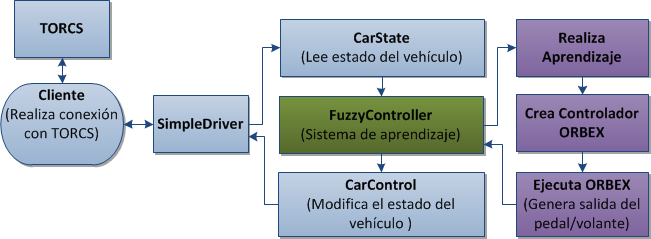
\includegraphics[width=0.6\linewidth]{figures/Diseno.png}
\caption{Esquema de ejecución de una prueba realizada con TORCS. Las clases en azul son las que vienen con TORCS, la clase verde fue la que se desarrolló y en morado se indica el funcionamiento de dicha clase}
\label{fig:esqT}
\end{figure}     

Para la automatización del pedal del automóvil, se implementó el cálculo de cinco \textbf{métricas del estado del vehículo}, las cuales se presentan en la tabla \ref{tab:metricas}, para utilizarlas como variables de entrada deben ser especificadas en el archivo de configuración.

\begin{table}[htb]
\begin{tabular}{|c|p{7.5cm}|c|}
\hline 
\rowcolor[gray]{0.9} \textbf{Métrica} & {\hspace{2.5 cm} \textbf{Descripción}} & \textbf{Formula} \\ 
\hline \hline
Error & Error de velocidad en un instante $i$ & \parbox{4cm}{\vspace{1 mm} $\gls{error} = \gls{P(i)} - \gls{V(i)}$ \vspace{0.5 mm}} \\ 
\hline 
Derivada & Rapidez con la que varia el valor del error de velocidad con respecto al tiempo & \parbox{4cm}{\vspace{1 mm}$\gls{dedt} = \frac{\gls{error}-\varepsilon_v(i-1)}{\gls{t(i)}-t(i-1)}$\vspace{0.5 mm}} \\ 
\hline 
Integral & El área bajo la curva de la función error de velocidad en los últimos diez instantes de tiempo & \parbox{5.6cm}{\vspace{1 mm}$\gls{integrall} = \gls{summod}$} \\ 
\hline 
Aceleración & Aceleración del automóvil & \parbox{4cm}{\vspace{1 mm}$\gls{a(i)} = \frac{V(i)-V(i-1)}{t(i)-t(i-1)}$\vspace{0.5 mm}} \\ 
\hline 
Perfil & Utiliza el valor del perfil de velocidad & \\ 
\hline 
\end{tabular} 
\caption{Métricas implementadas en el sistema. Donde $P(i)$ es el valor del perfil de velocidad, $V(i)$ la velocidad del carro y $t(i)$ el tiempo en el instante $i$. }
\label{tab:metricas}
\end{table}

%\begin{itemize}
%\item \textbf{Error}: error de velocidad en un instante $i$ calculado como 
%\[\gls{error} = \gls{P(i)} - \gls{V(i)}\]
%Siendo $P(i)$ el valor del perfil de velocidad en el instante $i$, y $V(i)$ la velocidad del carro en el instante $i$. 
%\item \textbf{Derivada}: rapidez con la que varia el valor del error de velocidad con respecto al tiempo:
%\[ \gls{dedt} = \frac{\gls{error}-\varepsilon_v(i-1)}{\gls{t(i)}-t(i-1)} \] 
%\item \textbf{Integral}: área bajo la curva de la función error de velocidad en los últimos diez instantes de tiempo:
%\[ \gls{integrall} = \gls{summod} \]
%\item \textbf{Aceleración}: aceleración del automóvil:
%\[ \gls{a(i)} = \frac{V(i)-V(i-1)}{t(i)-t(i-1)} \]
%\item \textbf{Perfil}: utiliza el valor del perfil de velocidad.
%\end{itemize}

El proceso cliente crea un nuevo objeto {\tt FuzzyController}, el cual se encarga tanto de todo el sistema de aprendizaje, como de la ejecución y configuración del controlador difuso definido por la librería \gls{ORBEX}. La clase {\tt FuzzyController} se inicializa con las variables mostradas en la tabla \ref{tab:fuzzycontroller}. 
%El constructor para crear una instancia de {\tt FuzzyController} es el siguiente:


\begin{table}[htb]
	\centering
		\begin{tabular}{|c|c|}
			\hline
			\rowcolor[gray]{0.9} \textbf{Campo} & \textbf{Descripción} \\ \hline \hline
			\textit{entries} & Número de entradas que se vana a pasar \\ \hline
			\textit{ets} & Número de etiquetas por cada variable de entrada \\ \hline
			\textit{rs1} & Rango inferior por cada variable de entrada \\ \hline
			\textit{rs2} & Rango superior por cada variable de entrada \\ \hline
			\textit{metrics} & Lista de métricas a utilizar \\ \hline
			\textit{ctte} & Constante de normalización (sección \ref{sec:aprendizajeL})\\ \hline
			\textit{size\_c} & Tamaño del ciclo a utilizar (sección \ref{sec:aprendizajeG}) \\ \hline
			\textit{control} & Genera un fichero de control si es verdadero \\ \hline
		\end{tabular}
		\caption{Variables utilizadas por la clase {\tt FuzzyController}.}
		\label{tab:fuzzycontroller}
\end{table}


%\begin{alltt}
%FuzzyController (
%    int entries, //número de entradas que se vana a pasar.
%    int *ets, //número de etiquetas por cada variable de entrada.
%    double *rs1, //rango inferior por cada variable de entrada.
%    double *rs2, //rango superior por cada variable de entrada.
%    string *metrics, //Lista de métricas a utilizar.
%    double ctte = 100, //Constante de normalización.
%    int size_c = 500, //Tamaño del ciclo a utilizar (sección \ref{sec:aprendizajeG}).
%    bool control = false //Genera un fichero de control si es verdadero.
%)
%\end{alltt}

{\tt FuzzyController} posee implementado el cálculo de los valores de las métricas que se definieron en el archivo de configuración, al igual que genera el archivo {\tt Controlador.ORB} que utiliza la librería \gls{ORBEX}, y \textbf{cinco archivos de salida},  presentados en la tabla \ref{tab:logs}.

\begin{table}[htb]
	\centering
\begin{tabular}{|l|p{12 cm}|}
\hline 
\rowcolor[gray]{0.9} \textbf{Nombre} & \textbf{Descripción} \\ \hline \hline
Log\_controller & Cada columna posee los valores correspondientes al estado del carro y del controlador difuso por cada iteración, como por ejemplo: el número de la iteración, valor del pedal (valor de salida de \gls{ORBEX}), velocidad y aceleración del automóvil, perfil de velocidad, variables de entrada, número de etiquetas, etc. \\ 
\hline 
Log\_etiquetas & Posee el grado de activación de las etiquetas correspondientes a las variables de entrada en cada iteración (referirse a la sección \ref{sec:orbex}) \\ 
\hline 
Log\_reglas & Posee el grado de activación de las reglas del controlador difuso en cada iteración \\ 
\hline 
Los\_singletons & Posee el valor de los singletons en cada iteración \\ 
\hline 
Log\_trapecios & Posee las coordenadas correspondientes a cada trapecio \\ 
\hline 
\end{tabular} 
\caption{Archivos de salida que se implementaron.}
\label{tab:logs}
\end{table}

%\begin{itemize}
%\item Log\_controller: en cada columna posee los valores correspondientes al estado del carro y del controlador difuso por cada iteración, como por ejemplo: el número de la iteración, valor del pedal (valor de salida de \gls{ORBEX}), velocidad y aceleración del automóvil, consigna de velocidad, variables de entrada, número de etiquetas, etc.
%\item Log\_etiquetas: posee el grado de activación de las etiquetas correspondientes a las variables de entrada en cada iteración.
%\item Log\_reglas: posee el grado de activación de las reglas del controlador difuso en cada iteración.
%\item Los\_singletons: posee el valor de los singletons en cada iteración.
%\item Log\_trapecios: posee las coordenadas correspondientes a cada trapecio.
%\end{itemize}


\section{Aprendizaje local} 
\label{sec:aprendizajeL}


El aprendizaje local consiste en \textbf{modificar los consecuentes de las reglas}, con la finalidad de que el sistema realice un seguimiento más preciso de la señal de referencia (en el caso del control de los pedales, la señal es el perfil de velocidad), y está basado en la evaluación del estado actual del automóvil y la corrección de las reglas responsables por alcanzar dicho estado. 

En la figura \ref{fig:esquemaL} se presenta un esquema del aprendizaje local de acuerdo a lo realizado en esta sección. Cuando indicamos que las acciones deben ser más altas o más bajas, significa que el impacto que generan las reglas que se activaron en la salida del pedal, no generan el comportamiento deseado, por lo que se deben aumentar o disminuir, según sea el caso, los singletons de dichas reglas. Nos referimos a que las acciones son adecuadas, cuando el controlador logra mantener el error de velocidad en cero, o cuando el controlador, logra que el error de velocidad vaya creciendo o reduciéndose para alcanzar al cero, mientras la aceleración del vehículo se encuentra en un rango establecido. 

\begin{figure}[!htb]
\centering
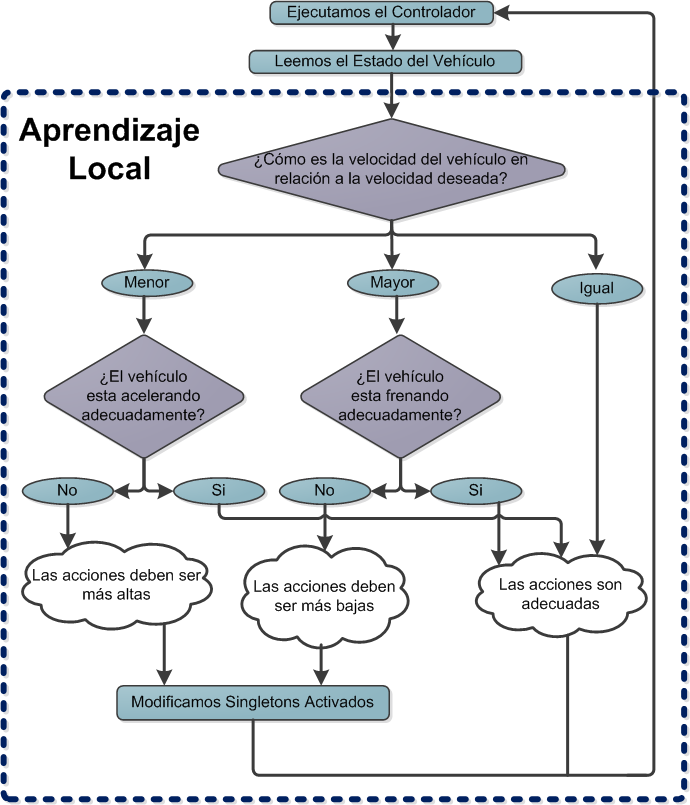
\includegraphics[width=0.75\linewidth, height= 10 cm]{figures/EsquemaLocal.png}
\caption{Esquema de funcionamiento de aprendizaje local.}
\label{fig:esquemaL}
\end{figure}  

Suponiendo una iteración del controlador, en el instante $t-1$ con un valor de referencia $P(t-1)$ (velocidad que se desea alcanzar) se obtiene un valor para el pedal. Al aplicarse dicho valor al carro, se alcanza la velocidad $V(t)$, en el caso de que $V(t) < P(t-1)$ significa que el valor del pedal para el instante $t$, debió haber sido mayor, de igual manera si $V(t) > P(t-1)$ implica que el valor del pedal fue demasiado elevado. En ambos casos, se debe corregir únicamente, los singletons correspondientes a aquellas reglas que se activaron para obtener el valor de salida del pedal, ya que son las responsables de que el vehículo alcanzara ese estado. La modificación de los singletons viene dada por la siguiente expresión:

\begin{equation}\label{eq:single}
\gls{s(t)} = s(t-1) + \frac{P(t-1)-V(t)}{\gls{Cte}}*\gls{mu_{i}(t-1)}
\end{equation}

\noindent, donde $s(t-1)$ es el valor del singleton en el instante $t-1$, $\mu_{i}(t-1)$ es el grado de activación de la regla $i$ en el instante $t-1$ y $Cte$ es una constante de normalización previamente definida. 

En todas las pruebas que se realizaron, los singletons fueron inicializados en cero, sin embargo el sistema puede utilizarse para ajustar los singletons de las reglas que utilicen controladores que hayan sido previamente configurados, bien sea por el mismo sistema de aprendizaje, o a partir de maquinas de aprendizaje que realicen un aprendizaje supervisado.


\subsection{Elección de la constante de normalización}


Se realizaron simulaciones en las cuales se probaron distintos valores de la constante de normalización, y fueron variándose el número de etiquetas por entrada, con la finalidad de elegir un valor adecuado para la constante. Como variables de entrada se utilizaron el error y la derivada del error, en los rangos [-25,25] y [-8,8] respectivamente, las funciones de pertenencia de cada variable de entrada se variaron desde 2 hasta 7 en cada corrida, los valores de constante utilizados fueron 50, 100 y 150. 

\begin{figure}[htb]
\centering
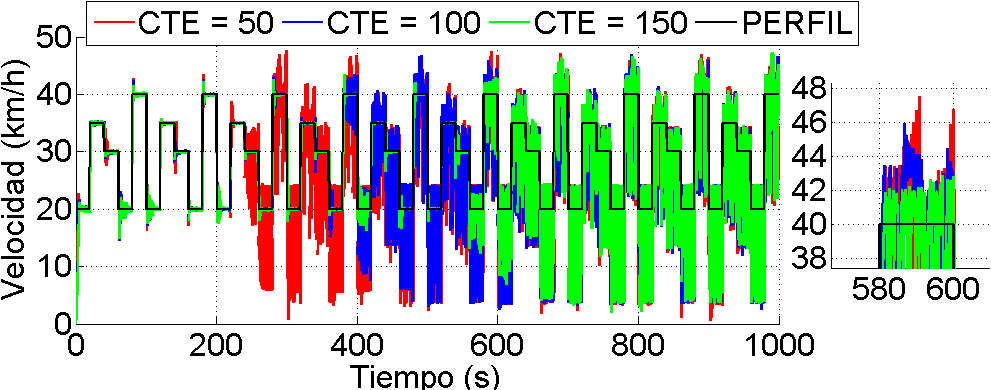
\includegraphics[width=0.6\linewidth,type=png,ext=.png,read=.png]{figures/tresC}
\caption{Comparación de simulaciones con distintos valores de la constante, utilizando 5 etiquetas por variable de entrada.}
\label{fig:tresC}
\end{figure} 



Al analizar los resultados de las distintas simulaciones, \textbf{se decidió por utilizar 100} como valor para la constante de normalización, en la figura \ref{fig:tresC}, se observa que entre 100 y 150, la diferencia no es tan notable, mientras que con 50 se observan oscilaciones muy grandes de la velocidad. Utilizar un valor como 50 o más pequeño resultaría en modificaciones muy grandes a los singletons, lo cual dificultaría las tareas de ajustes de algunas magnitudes como la aceleración, en cambio a medida que se va aumentando el valor de la constante de normalización, se va haciendo más lento el proceso de aprendizaje, debido a que se van haciendo más pequeños las modificaciones a los singletons, necesitando una cantidad mayor de ejecuciones del sistema para alcanzar una configuración aceptable.

Las grandes oscilaciones que se observan en la figura \ref{fig:tresC} un poco antes del segundo 400, se pensó que ocurrían debido a que los singletons se modificaban en cada iteración, y que se llegaba a un punto en el cual los cambios eran sencillamente muy grandes, por lo que obteníamos unos valores muy extremos para el pedal.


%\begin{figure}[htb]
%\centering
%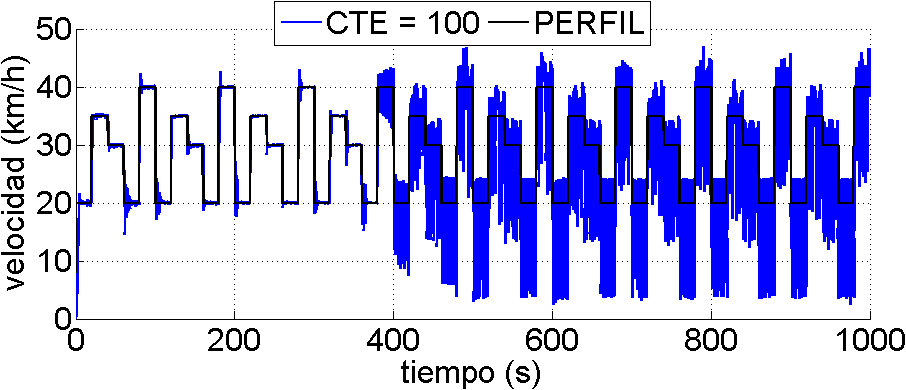
\includegraphics[width=0.8\linewidth,type=png,ext=.png,read=.png]{figures/ctte100}
%\caption{Simulación con el valor de la constante elegida.}
%\label{fig:ctte100}
%\end{figure} 

\subsection{Condicionamiento de la modificación de singletons}
\label{subsec:condicionamiento}


Con la finalidad de variar el valor de los singletons lo menos posible, se condicionó esta acción. Se establecieron \textbf{dos casos formados por tres reglas cada uno}, si ninguno de los dos se cumple, modificamos los singletons. Los casos se presentan a continuación:



\begin{itemize}
\item Caso 1: $V(i) < P(i)$, $a(i) > 0$ y $a(i) < \gls{a_c}+2$.
%\begin{itemize}
%\item $V(i) < P(i)$ : la velocidad del automóvil es menor a la velocidad que queremos alcanzar.
%\item $a(i) > 0$ : la aceleración del automóvil es positiva.
%\item $a(i) < a_c+2$ : la aceleración del automóvil es menor a la aceleración de confort más dos.
%\end{itemize}
\item Caso 2: $V(i) > P(i)$, $a(i) < 0$ y $a(i) > -a_c - 2$.
%\begin{itemize}
%\item $V(i) > P(i)$ : la velocidad del automóvil es mayor a la velocidad que queremos alcanzar.
%\item $a(i) < 0$ : la aceleración del automóvil es negativa.
%\item $a(i) > -a_c - 2$ : la aceleración del automóvil es mayor al negativo de la aceleración de confort menos dos.
%\end{itemize}
\end{itemize}

El \textit{Caso 1} representa la situación en que la velocidad del automóvil es menor a la velocidad que se desea alcanzar, la aceleración del automóvil es positiva y la aceleración del automóvil es menor a la aceleración de confort más dos. Mientras que el \textit{Caso 2} representa la situación especular. 

\textbf{La aceleración de confort} ($a_c$), es aquella a partir de la cual el cambio de velocidad genera una sensación desagradable en las personas. Se utilizó un valor de 8 km/h/s como aceleración de confort. El propósito del condicionamiento, es llegar a un punto en el cual se alcance el aprendizaje necesario, para poder procesar cualquier perfil de velocidad sin realizar modificaciones bruscas a los singletons.

\begin{figure}[htb]
\centering
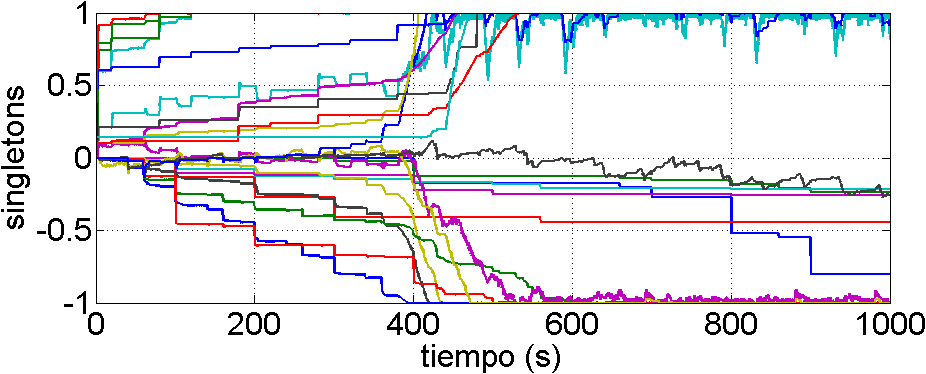
\includegraphics[width=0.5\linewidth,type=png,ext=.png,read=.png]{figures/421single1}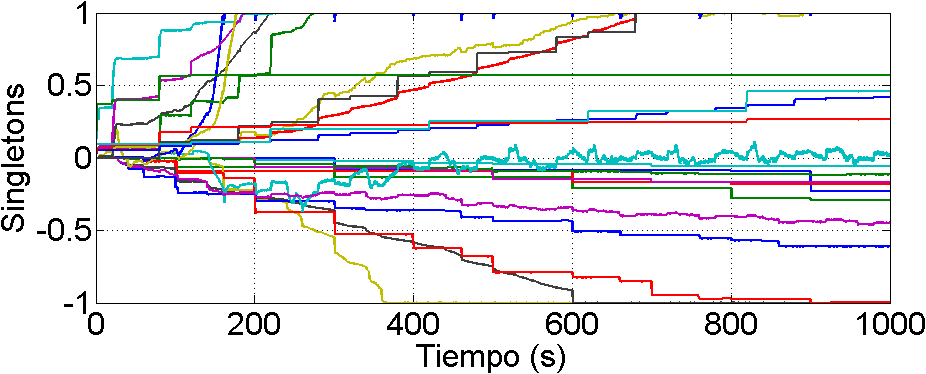
\includegraphics[width=0.5\linewidth,type=png,ext=.png,read=.png]{figures/421single2}
\caption{Singletons sin el condicionamiento (izquierda) y con el condicionamiento (derecha). Cada línea de color representa el valor de los singleton (consecuente de las reglas) a lo largo de la ejecución.}
\label{fig:421single2}
\end{figure} 

En la figura \ref{fig:421single2} se puede ver cómo varían los singletons en una ejecución del aprendizaje sin utilizar el condicionamiento de aceleración (izquierda) y utilizándolo (derecha). Cuando no se utiliza el condicionamiento algunos singletons son modificados repetidamente en pequeños espacios de tiempo, lo que resulta en oscilaciones cortas en las líneas que los representan; en cambio, cuando es utilizado se obtienen líneas más suaves, ya que al momento de modificarse los singletons se realizan principalmente uno o dos cambios seguidos.

Tratando de adecuar la aceleración del automóvil, para evitar un comportamiento violento, se hizo un \textbf{nuevo ajuste} luego de aplicada la fórmula de modificación de singletons. En caso de que la aceleración sea mayor a la aceleración de confort, se resta al singleton el 10\% del grado de activación que tuvo, mientras que si es menor al negativo de la aceleración de confort, se suma 10\% del grado de activación. Como el rango de los singletons es [-1,1], se debe garantizar que los valores se encuentren contenidos en él. 

Con este método se realizaron diversas simulaciones, para las cuales se utilizaron el valor de constante seleccionado anteriormente ($Cte=100$) y dos valores de entrada (\textit{error} y \textit{derivada}), a los que se les fueron variando sus respectivos números de etiquetas en cada prueba. En todas las pruebas se encontró el comportamiento que se presenta en la figura \ref{fig:loco100}, correspondiente a una simulación con cinco etiquetas por cada entrada.

\begin{figure}[htb]
\centering
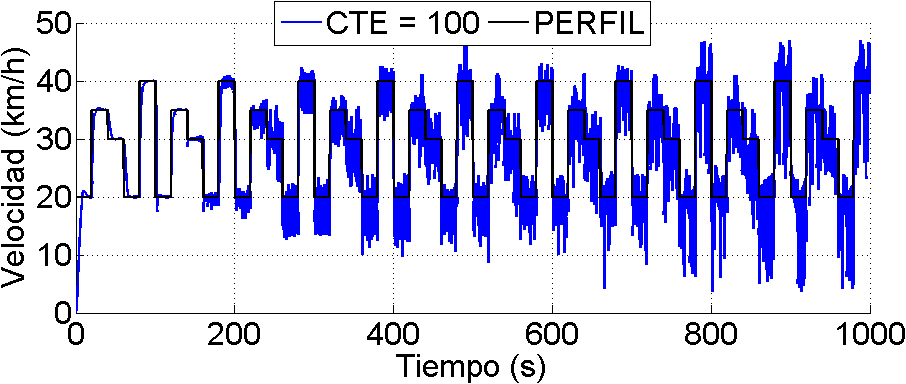
\includegraphics[width=0.6\linewidth,type=png,ext=.png,read=.png]{figures/loco100}
\caption{Simulación con el condicionamiento de singletons implementado.}
\label{fig:loco100}
\end{figure} 

Al ver que el problema de las oscilaciones grandes no se resolvía con el condicionamiento de la modificación de singletons, se hizo un análisis de la estructura del programa y la formulación del problema. Se encontró que el error se produce porque \textbf{la variación de singletons se realiza tras ejecutar el controlador \gls{ORBEX}}, y no luego de pasar el valor del pedal al carro y recibir los valores actualizados del estado del vehículo, por lo que se realizaban todos los cálculos y comparaciones, utilizando los valores de aceleración y velocidad correspondientes a la iteración anterior.

Al realizar la corrección de los consecuentes justo después de ejecutarse el controlador no se estaba aplicando la expresión \ref{eq:single}, sino que realmente se aplicaba la siguiente:
\[ s(t) = s(t-1) + \frac{P(t-1)-V(t-1)}{C}*\mu_{i}(t-1)\]

Como se aprecia en la figura \ref{fig:buenoCtte100}, al \textbf{reestructurar el código} para que se realizaran las modificaciones a los singletons luego de que se aplicara el nuevo valor del pedal, de forma tal que la formula utilice el valor de velocidad correspondiente, se eliminaron las oscilaciones bruscas que ocurren un poco antes del instante 400, y se observa un comportamiento más sutil.

\begin{figure}[htb]
\centering
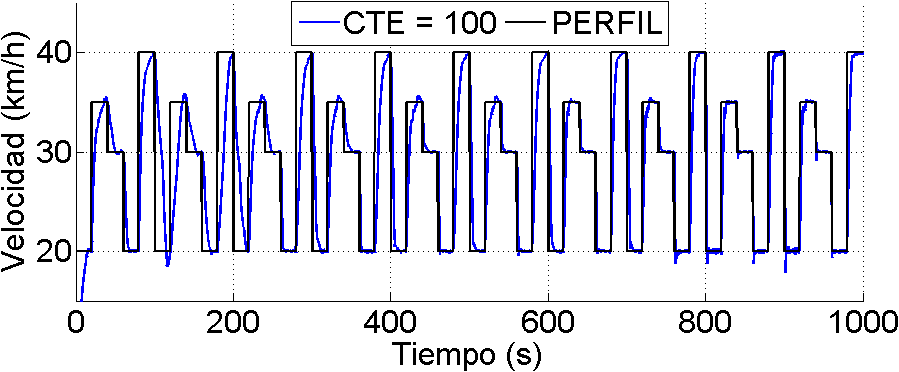
\includegraphics[width=0.6\linewidth,type=png,ext=.png,read=.png]{figures/buenoCtte100}
\caption{Simulación con reestructuración del código de modificación.}
\label{fig:buenoCtte100}
\end{figure} 

Durante la ejecución de las simulaciones se obtuvieron valores de aceleración muy por encima de lo adecuado, pero se decidió implementar primero el aprendizaje global, antes que buscar maneras para mejorar los valores desde la etapa local, esperando obtener mejoras con la implementación de la nueva etapa.


\section{Aprendizaje global}
\label{sec:aprendizajeG}

En esta etapa, el objetivo es evaluar el comportamiento que ha mostrado el controlador, y decidir si es necesario \textbf{modificar la topología} del mismo, ya sea modificando la posición de la base superior de los trapecios, o insertando etiquetas o funciones de pertenencia nuevas. En la figura \ref{fig:esquemaG}, se presenta un esquema con el aprendizaje global, de acuerdo a lo realizado en esta sección.

\begin{figure}[!htb]
\centering
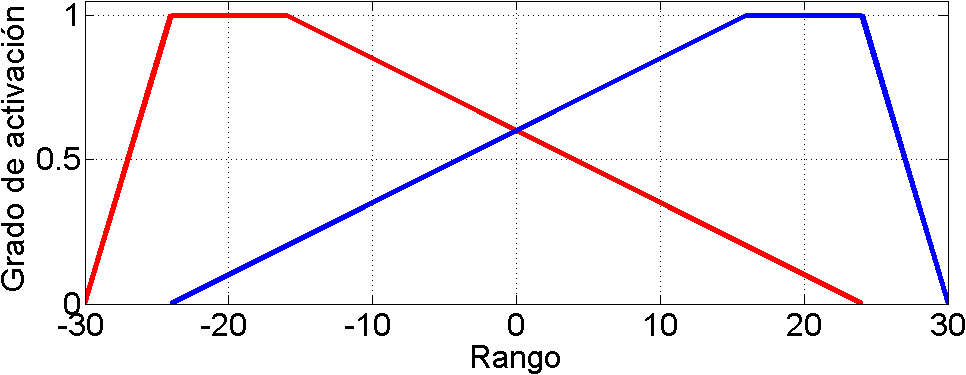
\includegraphics[width=0.35\linewidth]{figures/2.png} \hspace{0.5cm} 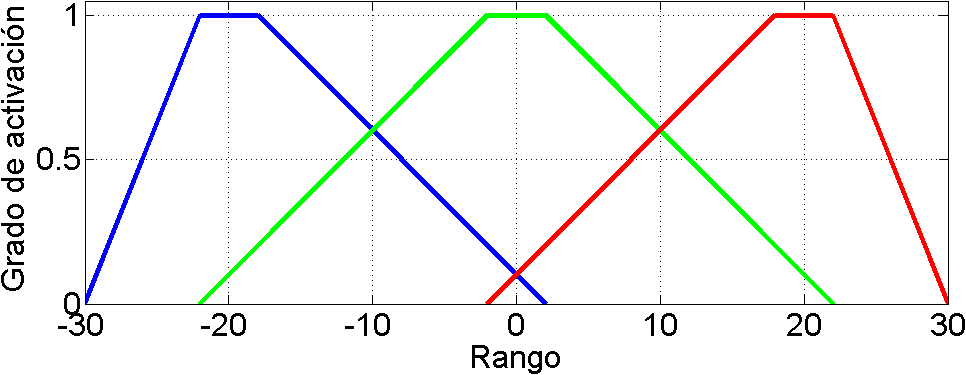
\includegraphics[width=0.35\linewidth]{figures/3.png}
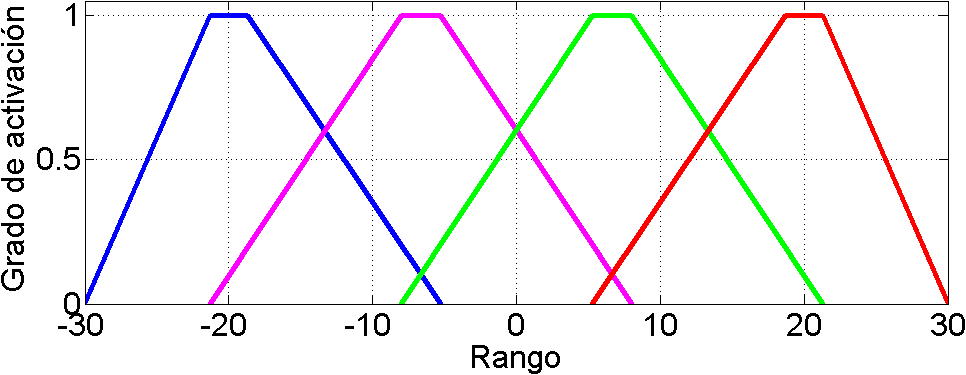
\includegraphics[width=0.35\linewidth]{figures/4.png} \hspace{0.5cm} 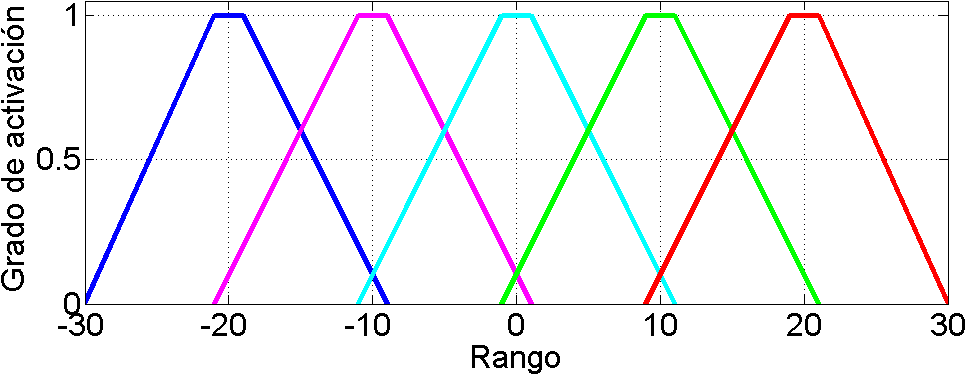
\includegraphics[width=0.35\linewidth]{figures/5.png}
\caption{Topología de un controlador, que utiliza funciones de pertenencia o etiquetas, con forma trapezoidal, igualmente distribuidas en un rango de [-20,20], con dos etiquetas (arriba izquierda), con tres etiquetas (arriba derecha), con cuatro etiquetas (abajo izquierda) y con cinco etiquetas (abajo derecha)}
\label{fig:trapeciosD}
\end{figure} 

El sistema se diseñó para trabajar con trapecios igualmente distribuidos, cada vez que se va a insertar una nueva etiqueta a alguna variable de entrada, se genera el nuevo grupo de trapecios y se colocan a lo largo del rango de la variable, como se aprecia en la figura \ref{fig:trapeciosD}. Los trapecios están colocados de manera que se pueda garantizar que cualquier valor de entrada estará cubierto como mínimo por dos trapecios.

\begin{figure}[!htb]
\centering
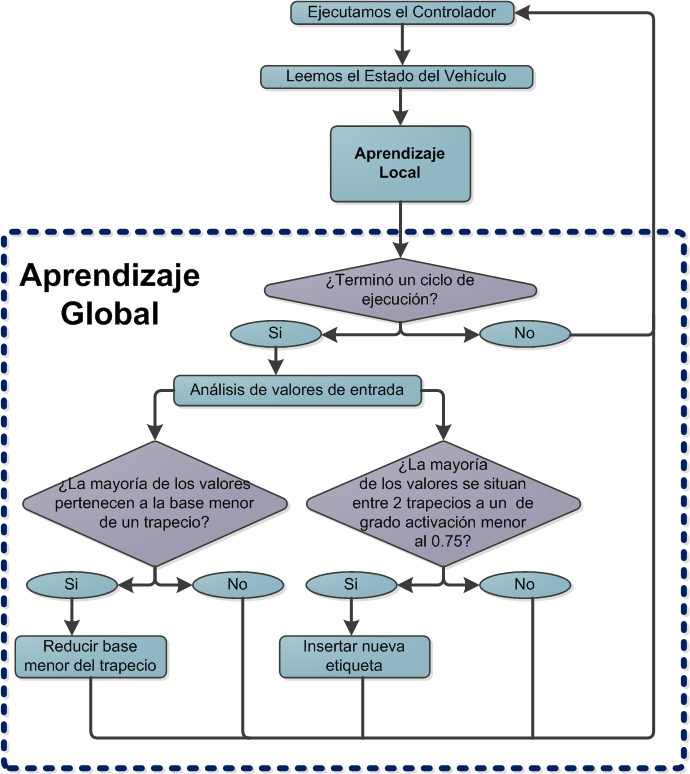
\includegraphics[width=0.75\linewidth, height = 10 cm]{figures/EsquemaGlobal.png}
\caption{Esquema de funcionamiento de aprendizaje global.}
\label{fig:esquemaG}
\end{figure} 

Se comienza el aprendizaje global dividiendo el rango de cada variable de entrada entre la mitad del tamaño de la base menor de un trapecio, de tal manera que la base menor de cada trapecio este cubierta por lo menos por dos subrangos. En caso que el número de subrangos que se generan de la división es par, se aumenta dicho número en uno, ya que si dividimos entre un número impar, garantizamos tener un subrango en cual el punto medio sea el cero.

Cada vez que se ejecuta el controlador, se busca a que subrango pertenecen los valores de entrada, y se aumenta en uno un contador que corresponde al número de valores de entrada que han pertenecido a dicho subrango. 

Se define un \textbf{ciclo de ejecución} como la evaluación de un cierto número de iteraciones del controlador, el tamaño de estos se especifica en la variable \textit{size\_c} del constructor de la clase \textit{FuzzyController}. Cada vez que se termina un ciclo, se ejecuta la etapa de aprendizaje global, se comienza por determinar cuáles son los dos subrangos con mayor valor en su contador. Utilizando el punto medio de los dos subrangos, se busca a cuales trapecios pertenecen y se determina si se encuentran en alguno de estos dos casos:

\begin{itemize}
\item Ambos puntos pertenecen a la base menor del mismo trapecio.
\item Ambos puntos pertenecen al mismo lado del trapecio, y se encuentran a un nivel de activación menor al 75\%
\end{itemize} 

En caso de pertenecer a la base menor del mismo trapecio, \textbf{se reduce la base menor}  de dicho trapecio en un 80\% y se reinician los contadores de los subrangos. Al reducir la base menor, se evita que la gran mayoría de los valores de entrada posean el mismo grado de activación, obteniendo un controlador más específicos. 

\begin{figure}[htb]
\centering
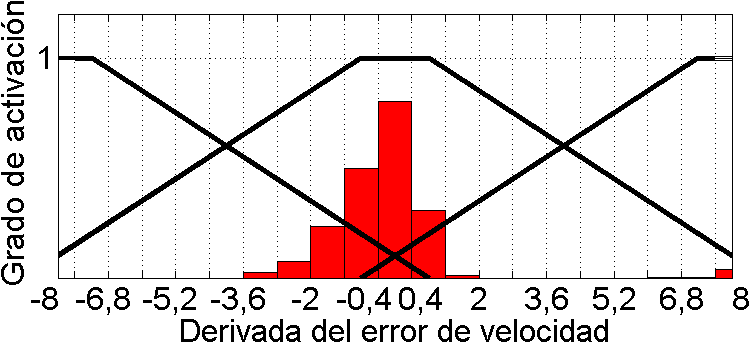
\includegraphics[width=0.45\linewidth,type=png,ext=.png,read=.png]{figures/label11}\hspace{0.5cm} 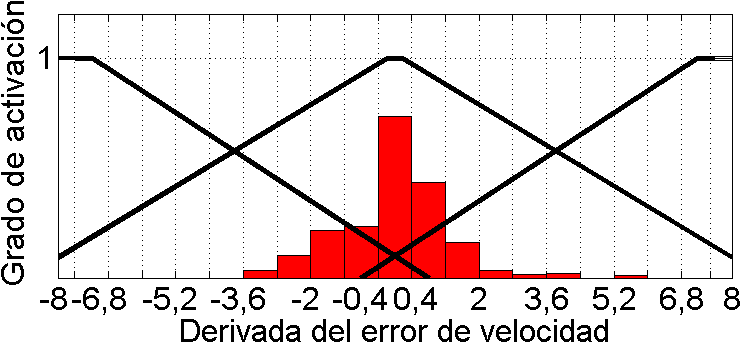
\includegraphics[width=0.45\linewidth,type=png,ext=.png,read=.png]{figures/label12}
\caption{Histograma del error de velocidad obtenido en un ciclo, con sus respectivas funciones de pertenencia antes de realizar el ajuste global (izquierda) y tras realizar el ajuste global (derecha).}
\label{fig:label11}
\end{figure} 

En la figura \ref{fig:label11} (izquierda) se puede observar que la gran mayoría de los valores de entrada obtenidos de la derivada del error en un ciclo, se encuentran alrededor del cero, y dada la manera en la que están distribuidos los trapecios, ese rango de valores pertenecen a la base menor del trapecio ubicado en el medio. De acuerdo a las reglas colocadas, se debe reducir la base en un 80\%, como se aprecia en la figura \ref{fig:label11} (derecha), correspondiente al ciclo de ejecución siguiente.

%\begin{figure}[htb]
%\centering
%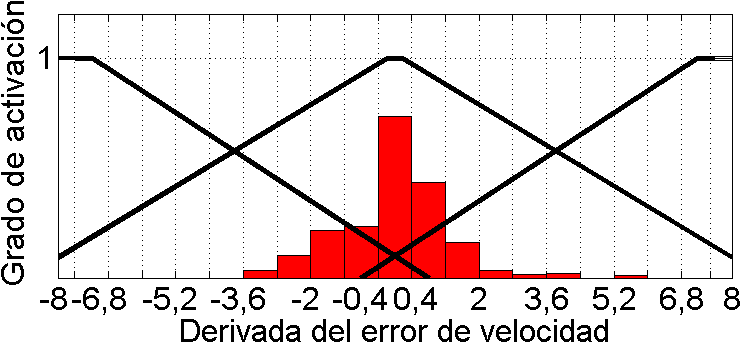
\includegraphics[width=0.8\linewidth,type=png,ext=.png,read=.png]{figures/label12}
%\caption{Topología luego de la reducción de la base menor del trapecio ubicado en el medio.}
%\label{fig:label12}
%\end{figure} 

Si ambos puntos se encuentran en el mismo lado del trapecio y a un nivel de activación menor al 75\%, se procede a \textbf{insertar un nueva función de pertenencia} de la siguiente manera: se genera la nueva cantidad de trapecios uniformemente distribuidos para esa entrada, se actualiza el número de etiquetas y se recalculan el número de reglas, subrangos, singletons, asignándole cero a estos últimos. 

\begin{figure}[h]
\centering
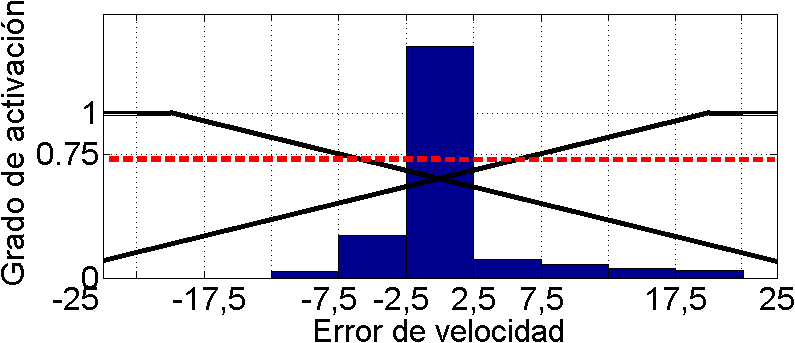
\includegraphics[width=0.45\linewidth,type=png,ext=.png,read=.png]{figures/label21}\hspace{0.5cm} 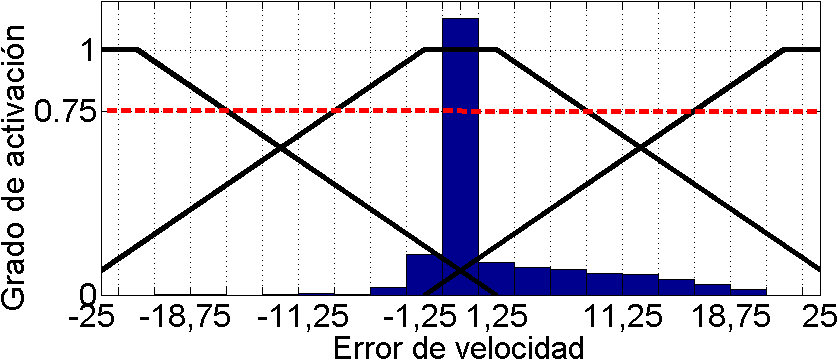
\includegraphics[width=0.45\linewidth,type=png,ext=.png,read=.png]{figures/label22}
\caption{Histograma de la derivada del error en un ciclo, con sus respectivas funciones de pertenencia antes de realizar el ajuste global (izquierda) y tras el ajuste global (derecha).}
\label{fig:label21}
\end{figure} 

El caso en el cual se inserta una nueva función de pertenencia, se puede apreciar en la figura \ref{fig:label21} (izquierda). Los dos subrangos con mayor número de elementos, se encuentran a un nivel de activación menor al 75\%, por lo que se agrega una función de pertenencia nueva y se recalculan los trapecios asociados a dichas funciones, para la ejecución del ciclo siguiente, como se ve en la figura \ref{fig:label21} (derecha). 

%\begin{figure}[h]
%\centering
%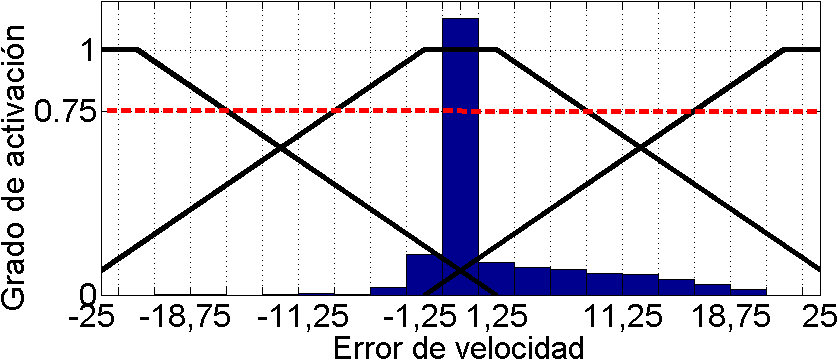
\includegraphics[width=0.8\linewidth,type=png,ext=.png,read=.png]{figures/label22}
%\caption{Topología luego de la inserción de una nueva función de pertenencia.}
%\label{fig:label22}
%\end{figure} 



\section{Ajuste de la aceleración}
\label{sec:ajuste}

En las simulaciones realizadas, se encontró que el vehículo alcanzaba unos niveles de aceleración (tanto positiva como negativa) muy por encima de lo deseable, resultado de los elevados valores que se transmitían al pedal a la hora de encontrarse con un cambio en el perfil de velocidad. Esta situación ocurría ya que el controlador buscaba alcanzar el nuevo valor con la mayor rapidez posible, de manera que el error de velocidad se vuelva cero. 

Ésto se ilustra en la figura \ref{fig:frenaso}, donde se muestra la aceleración obtenida por el vehículo en una de las simulaciones. En ella puede verse que en el instante 400, momento cuando termina el cuarto ciclo (cada ciclo dura 100 segundos, sección \ref{subsec:diseno}) y ocurre el cambio de 40 km/h a 20 km/h, la aceleración sobrepasa el valor de -10 km/h/s, que es el límite aceptable establecido para esta magnitud. A partir de ese momento, se evidencia un aumento muy brusco a la hora de terminar los ciclos, dado que el controlador, para reducir rápidamente la velocidad, manda una señal muy fuerte al pedal. En los primeros tres ciclos no se evidencia este fenómeno, ya que en estos ciclos se realizan las modificaciones a la topología del controlador, que finalizan con la reinicialización de los singletons. 

\begin{figure}[h]
\centering
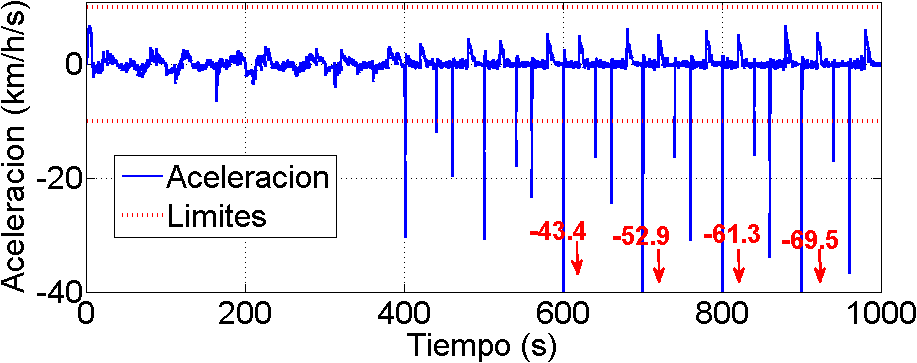
\includegraphics[width=0.6\linewidth,type=png,ext=.png,read=.png]{figures/frenaso}
\caption{Aceleración del vehículo.}
\label{fig:frenaso}
\end{figure} 

Para ajustar el cambio de aceleración, se modificó la etapa de aprendizaje local, y se agregó unos cambios correspondientes al comportamiento de los pedales del vehículo, los cuales se explican en las secciones \ref{subsec:ajusteS} y \ref{sec:ajusteP} respectivamente. En la figura \ref{fig:esquemaA} se presenta un esquema de como queda el sistema de aprendizaje, luego de aplicarse los nuevos ajustes.  

\begin{figure}[htb]
\centering
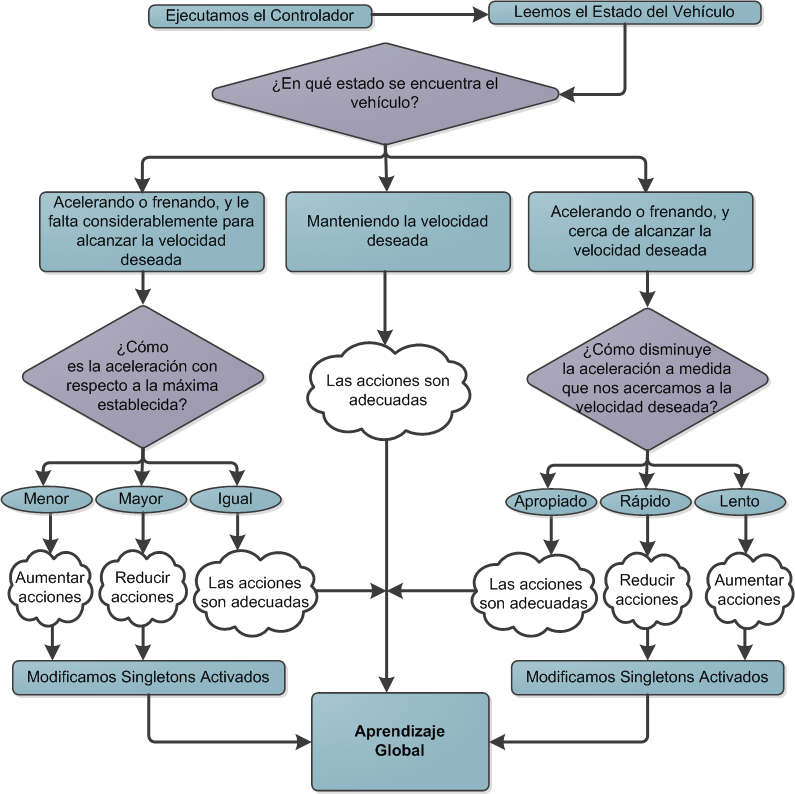
\includegraphics[width=0.85\linewidth,height = 10 cm]{figures/EsquemaAjustes.png}
\caption{Esquema de funcionamiento de aprendizaje local luego de los ajustes.}
\label{fig:esquemaA}
\end{figure}

\subsection{Ajuste a la modificación de singletons}
\label{subsec:ajusteS}


En la sección \ref{subsec:condicionamiento}, se establecieron dos condiciones para que se realice la \textbf{modificación de los singletons} y poder controlar mejor el comportamiento del automóvil, las cuales se cambiaron por unas más específicas. Se identificaron varias situaciones para las cuales se van a realizar dichas modificaciones.

\textbf{Si el error de velocidad es positivo ($velocidad<perfil$)} se debe acelerar para alcanzar la nueva consigna. Dependiendo de qué tan cerca se encuentra de alcanzar la velocidad deseada, se definen dos casos.

\begin{enumerate}
\item Si el error de velocidad es mayor al valor de la aceleración de confort ($\gls{error}>a_c$); el automóvil se encuentra en un estado favorable para alcanzar la aceleración máxima establecida. Tomando esto en consideración, la modificación de los singletons se establece según:
\begin{itemize}
\item $a(i) > a_c +2$ : el automóvil sobrepasó la aceleración máxima, por lo que se realiza una disminución al valor de los singletons, que viene dada por la siguiente expresión:
\begin{equation}\label{eq:sinMenos}
s(t) = s(t-1) - \frac{P(t-1)-V(t)}{C}*\mu_{i}(t-1)
\end{equation}
\item $a(i) < a_c -2$ : el automóvil no ha alcanzado la aceleración máxima, por lo que se realiza un aumento al valor de los singletons, el cual viene dado por:
\begin{equation}\label{eq:sinMas}
s(t) = s(t-1) + \frac{P(t-1)-V(t)}{C}*\mu_{i}(t-1)
\end{equation}
\item Si no se cumple ninguna de las condiciones anteriores, es decir, la aceleración del carro se encuentra en el intervalo [$a_c -2$,$a_c +2$], el vehículo se encuentra en el punto óptimo de aceleración, en el que no se realizan modificaciones.
\end{itemize}
 

\item En el caso donde $\gls{error} \leq a_c$, el carro debe ir disminuyendo progresivamente la aceleración a medida que se alcanza el valor de la consigna. De la misma manera como ocurre en el caso anterior:

\begin{itemize}
\item $a(i) > \gls{error}+2$ : el automóvil no ha disminuido lo suficiente la aceleración, por lo que se realiza una disminución al valor de los singletons, que viene dada por la expresión (\ref{eq:sinMenos}).
\item $a(i) < max(0,\gls{error}-2)$ : el automóvil ha disminuido demasiado la aceleración, por lo que se realiza un aumento al valor de los singletons, el cual viene dado por la expresión (\ref{eq:sinMas}). Se utiliza el máximo entre $0$ y $\gls{error}-2$, debido a que si se encuentra que $\gls{error}-2 < 0$, no se puede permitir que el automóvil tenga una velocidad menor que la deseada y se encuentre frenando, en este caso el rango que se permite de aceleración para el cual no se modifican los singletons queda de la siguiente manera [$0$, $\gls{error}+2$].

\item A medida que disminuye el error de velocidad, se deja un rango para la aceleración de [$\gls{error}-2$, $\gls{error}+2$], en el cual no se modifican los singletons.
\end{itemize}

\end{enumerate}


 
\textbf{Cuando el error de velocidad es negativo}, el vehículo debe frenar, se mantiene el mismo planteamiento que se utiliza en el caso anterior, ya que los casos que se presentan son análogos.

\begin{enumerate}
\item Si $\gls{error}<-a_c$, se busca alcanzar la aceleración negativa máxima, para lo cual se divide el problema en:
\begin{itemize}
\item $a(i) < -a_c -2$ : el automóvil está frenando demasiado, por lo que se realiza un ajuste a los singletons, dado por (\ref{eq:sinMenos}).
\item $a(i) > -a_c +2$ : el automóvil no desacelera lo suficiente, por lo que se aplica la expresión (\ref{eq:sinMas}) para ajustar los singletons.
\item Si no se cumple ninguna de las condiciones, los singletons no se modifican.
\end{itemize}


\item De igual manera que en el caso anterior, si $\gls{error} \geq -a_c$, se divide el problema en dos:
\begin{itemize}
\item $a(i) < \gls{error}-2$ : el automóvil sigue frenando muy fuerte, por lo que se realiza una disminución al valor de los singletons, que viene dada por la expresión (\ref{eq:sinMenos}).
\item $a(i) > min(0,\gls{error}+2)$ : el automóvil no disminuye la aceleración como se espera, por lo que se realiza un aumento al valor de los singletons, el cual viene dado por la expresión (\ref{eq:sinMas}). En este caso se utiliza el mínimo entre $0$ y $\gls{error}+2$, para evitar estar en una situación donde no se modifiquen los consecuentes, y se espera que el carro este frenando, pero en realidad se encuentre acelerando.
\item Nuevamente, si no se cumple ninguna de las condiciones, los singletons no se modifican.
\end{itemize}

\end{enumerate}


%En el cuadro \ref{tab:casosS} se presentan los casos de manera resumida.
%
%\begin{table}[htb]
%\centering
%\begin{tabular}{|p{2.5cm} | p{4.5cm} | p{4.5cm} | p{3cm} |}
%\hline
%\rowcolor[gray]{0.9} Caso 1   & $a(i)< a_c-2$              & $a(i) \in [ a_c-2$,$a_c+2]$ & $a(i) > a_c+2$ \\ \hline
%$ \varepsilon_v(i) > a_c $ & Expresión: (\ref{eq:sinMas}) & No se modifica & Expresión: (\ref{eq:sinMenos}) \\ \hline  \hline
%
%\rowcolor[gray]{0.9} Caso 2& $a(i)< max(0,\varepsilon_v(i)-2)$ & $a(i) \in [ \varepsilon_v(i)-2$,$\varepsilon_v(i)+2]$ & $a(i) > \varepsilon_v(i)+2)$ \\ \hline
%$ \varepsilon_v(i) \in [0$,$a_c] $ & Expresión: (\ref{eq:sinMas}) & No se modifica & Expresión: (\ref{eq:sinMenos}) \\ \hline \hline
%
%\rowcolor[gray]{0.9} Caso 3 & $a(i)< -a_c-2$              & $a(i) \in [ -a_c-2$,$-a_c+2]$ & $a(i) > -a_c+2$ \\ \hline
%$ \varepsilon_v(i) > -a_c $ & Expresión: (\ref{eq:sinMas}) & No se modifica & Expresión: (\ref{eq:sinMenos}) \\ \hline \hline
%
%\rowcolor[gray]{0.9} Caso 4& $a(i)< \varepsilon_v(i)-2$ & $a(i) \in [ \varepsilon_v(i)-2$,$\varepsilon_v(i)+2]$ & \raggedright $a(i)> $ $min( \varepsilon_v(i)+2)$,$0]$ \tabularnewline
% \hline
%$ \varepsilon_v(i)$ $\in [-a_c$,$0] $ & Expresión: (\ref{eq:sinMas}) & No se modifica & Expresión: (\ref{eq:sinMenos}) \\ \hline  
%
%\end{tabular}
%\caption{Casos correspondientes a la modificación de singletons}
%\label{tab:casosS}
%\end{table}

Este enfoque más específico permite mantener un control más delicado a la hora de cambiar la velocidad. Se busca imitar la forma de conducir de las personas, las cuales no aceleran a fondo hasta llegar a la velocidad que desean, si no que pisan el pedal hasta lograr una aceleración adecuada, y a medida que se van acercando a la velocidad a la que quieren llegar, sueltan lentamente el pedal del acelerador, para no sobrepasarse.


\begin{figure}[h]
\centering
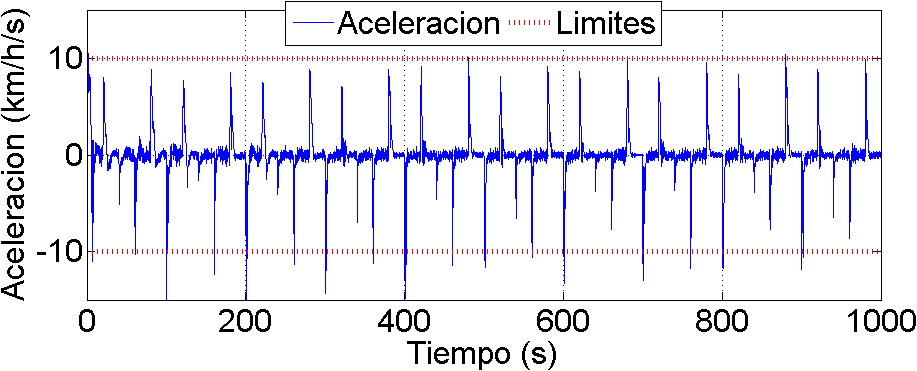
\includegraphics[width=0.6\linewidth,type=png,ext=.png,read=.png]{figures/freno4c}
\caption{Aceleración del vehículo, con el nuevo enfoque de modificación de singletons.}
\label{fig:freno4c}
\end{figure} 


En la figura \ref{fig:freno4c} se observa como la aceleración positiva alcanzó el máximo cuando le tocaba conseguir velocidades superiores, sobrepasando el límite solo en dos ocasiones, llegando a 10.42 km/h/s y 10.09 km/h/s, que son valores aceptables y no representan un problema mayor. 

Con respecto a los momentos donde se debía frenar, se logró reducir considerablemente los valores que se alcanzaban, aunque seguía sobrepasando el límite establecido, el mínimo al que llegó fue -21.80 km/h/s. Utilizando el otro enfoque, el mínimo que se alcanzó fue de -69.47 km/h/s y el comportamiento que presentó el controlador, indicaba que en el ciclo siguiente iba a ser mayor, mientras que en el nuevo, el mínimo se alcanzó en el segundo ciclo, cuando el controlador está realizando los ajustes a la topología, a partir de ese punto, a medida que avanza el aprendizaje, se fueron disminuyendo poco a poco los mínimos de aceleración.


\subsection{Ajustes del pedal}
\label{sec:ajusteP}


Cuando el valor de salida del controlador, que corresponde al pedal del controlador, cambia de signo, dependiendo del signo al que cambie, implica que \textbf{se cambió entre el pedal de aceleración y el de freno}. Este cambio no puede ser instantáneo, no se puede pasar de un valor positivo (acelerar) inmediatamente a uno negativo (frenar), ya que el objetivo es imitar la manera de conducir de las personas, por lo que se debe soltar completamente el pedal que se está utilizando, y luego presionar el otro. 

Tomando en cuenta este comportamiento, si se encuentra un cambio de signo en la salida del controlador, \textbf{se devuelve cero} como salida del pedal durante las iteraciones correspondientes a el cambio de pedal. Es importante no realizar ajuste a los singletons durante este tiempo, ya que el resultado que se devuelve y los valores obtenidos con esa salida, no corresponden a los singletons utilizados. Se establecieron tres iteraciones con salida cero para imitar el cambio de pedal.


En la figura \ref{fig:pedal002}, se observa un periodo de tiempo en el cual el carro debe frenar porque está pasando de 40 km/h a 20 km/h. Sin embargo se nota que hay dos instantes en los que el pedal pasa al lado positivo. Analizando el valor que adopta el pedal en estos dos instantes, se puede decir que son casi insignificantes, pero representan un comportamiento que no queremos que adopte el carro. No tiene sentido que mientras se esta frenando, se suelte el pedal correspondiente al freno, para pisar casi de manera imperceptible al acelerador, e inmediatamente continuar frenando. 

\begin{figure}[h]
\centering
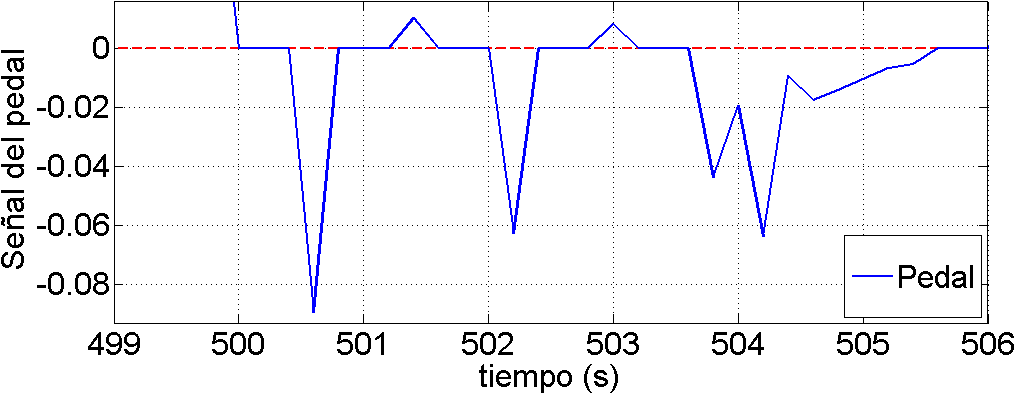
\includegraphics[width=0.6\linewidth,type=png,ext=.png,read=.png]{figures/pedal002}
\caption{Valores del pedal al pasar de 40 km/h a 20 km/h.}
\label{fig:pedal002}
\end{figure} 

Cuando se encuentren valores del pedal cuyo valor absoluto sea menor a 0.02, se retorna cero, ya que es un rango tan pequeño que los valores pertenecientes a él no inducen grandes cambios en el automóvil, y de esta forma se eliminan esos casos tan particulares.

El \textbf{último ajuste} que se realizó tuvo que ver nuevamente con la modificación de los singletons. Al analizar los resultados de las simulaciones, se encontró que los momentos en los cuales la aceleración alcanzó los valores más elevados, fueron aquellos en los que se estaba \textbf{en presencia de un cambio en el perfil de velocidad}. Cuando ocurre un cambio en el perfil, los valores de entrada cambian, el controlador que se encontraba a una velocidad constante con aceleración constante, pasa a encontrarse en una situación en la cual debe aumentar la aceleración, ya sea positiva o negativamente. 


El problema es que no se le da una oportunidad al controlador para tratar de alcanzar el nuevo valor de aceleración óptima, sino que se modifican los singletons instantáneamente siguiendo las reglas de la sección \ref{subsec:ajusteS}, las cuales indican que si se trata de alcanzar una velocidad, para que no se modifiquen los singletons, el vehículo  debe encontrarse en un cierto rango de aceleración. El automóvil para mantener una velocidad, debe mantener presionado el pedal del acelerador lo suficiente como para que esta no disminuya, resultando en una aceleración casi constante que oscila en un rango muy pequeño al rededor del cero, como podemos observar en la figura \ref{fig:aceCtte}. 

\begin{figure}[h]
\centering
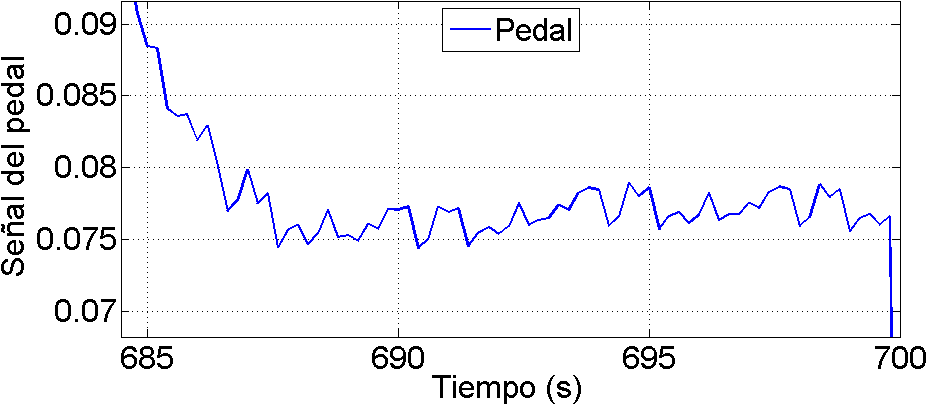
\includegraphics[width=0.5\linewidth,type=png,ext=.png,read=.png]{figures/pedalCtte}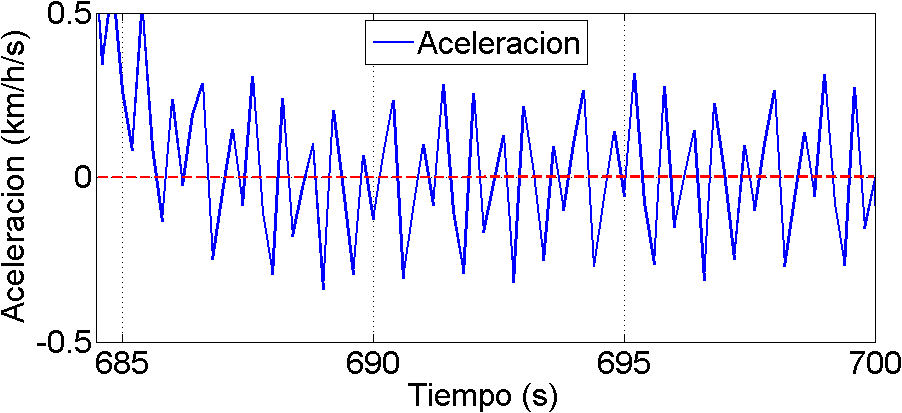
\includegraphics[width=0.5\linewidth,type=png,ext=.png,read=.png]{figures/aceCtte}
\caption{Valor del pedal (Izquierda) y aceleración del automóvil (derecha) en un tramo constante a 40 km/h.}
\label{fig:aceCtte}
\end{figure} 

Si el carro va manteniendo un velocidad constante y se genera un cambio de perfil, al comparar la aceleración actual con la óptima establecida para alcanzar la nueva velocidad, obtendremos que es necesario hacer un ajuste a los singletons, pero la mayoría de las veces el ajuste resulta ser demasiado elevado, ocasionando saltos muy grandes en la señal del pedal, y como el aumento de la aceleración negativa es más sensible a los cambios en los valores del pedal que la aceleración positiva, nos encontramos con los elevados valores en los momentos cuando se debe frenar. Para mejorar la situación, cada vez que nos encontramos con un cambio en los valores del perfil de velocidad, \textbf{dejamos que el controlador se ejecute, sin hacerle modificaciones a los singletons} durante un periodo de cinco iteraciones, de esta manera podemos probar si el controlador que se estaba utilizando para mantener la velocidad constante, se ajusta a la tarea de alcanzar la nueva velocidad.

\begin{figure}[h]
\centering
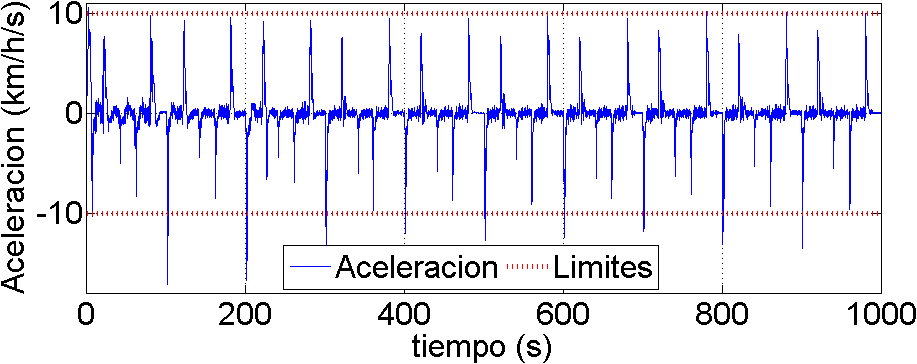
\includegraphics[width=0.6\linewidth,type=png,ext=.png,read=.png]{figures/acelFinal}
\caption{Aceleración del automóvil en un tramo constante a 40 km/h.}
\label{fig:acelFinal}
\end{figure}

Con el nuevo enfoque se logró reducir la aceleración mínima obtenida al momento de frenar de -21.80 km/h/s a -17.17 km/h/s. En la figura \ref{fig:acelFinal}, se observa que este valor se obtuvo en el primer cambio de 40 km/h a 20 km/h, y que luego de los tres primeros ciclos, al terminar los ajustes en la topología, los valores que se obtuvieron al realizar este cambio de velocidad, se encontraron entre -13 km/h/s y -11 km/h/s.
 
Con respecto a los singletons, como se muestra en la figura \ref{fig:singleFin}, se logró obtener un comportamiento muy estable. Luego de la etapa de modificación de la topología, llegó un punto en el que los singletons presentaban un comportamiento casi constante, caracterizado por pequeñas oscilaciones.


\begin{figure}[h]
\centering
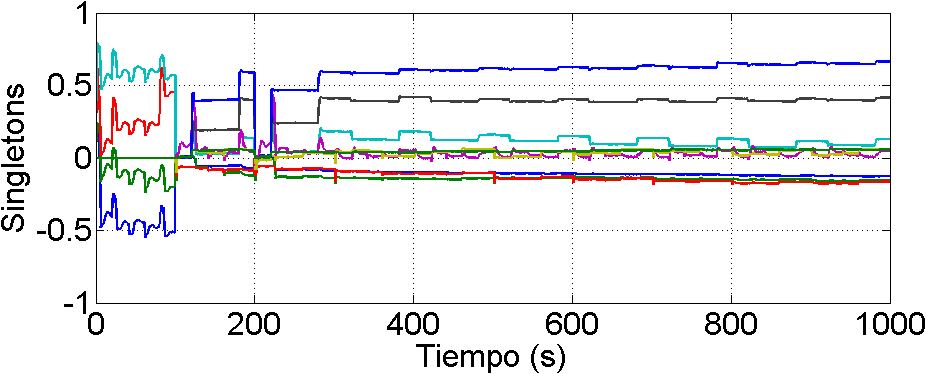
\includegraphics[width=0.6\linewidth,type=png,ext=.png,read=.png]{figures/singleFin}
\caption{Comportamiento de los singletons luego de aplicados todos los ajustes al sistema. Cada línea de color representa el valor de un singletons a lo largo de la ejecución.}
\label{fig:singleFin}
\end{figure} 


\begin{figure}[h]
\centering
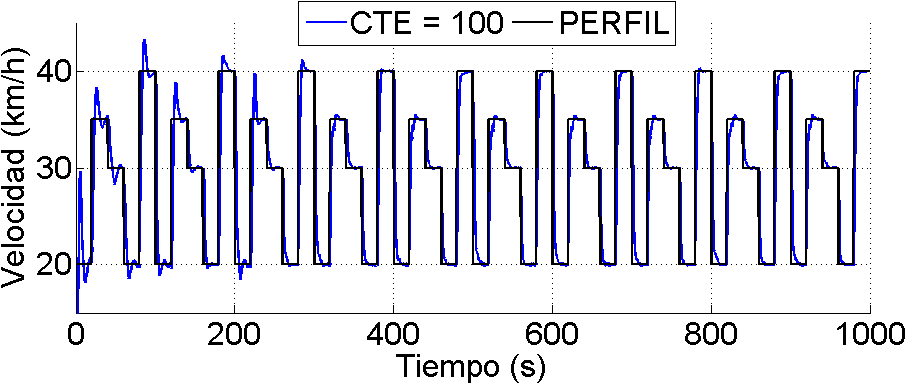
\includegraphics[width=0.6\linewidth,type=png,ext=.png,read=.png]{figures/velFin}
\caption{Velocidad del carro luego de aplicados todos los ajustes al sistema.}
\label{fig:velFin}
\end{figure} 



